%%%%%%%%%%%%%%%%%%%%%%%%%%%%%%%%%%%%%%%%%%%%%%
%                insertmeeting
% 1) Title (something creative & funny?)
% 2) Date (MM/DD/YYYY)
% 3) Location (ex. Hagerty High School)
% 4) People/Committees Present 
% 5) Picture 
% 6) Start Time & Stop Time (ex. 12:30AM to 4:30PM)
%%%%%%%%%%%%%%%%%%%%%%%%%%%%%%%%%%%%%%%%%%%%%%
\insertmeeting 
	{Carbon Fiber Is So Hot} 
	{02/10/22} 
	{Hagerty High School}
	{James, Jensen, Samantha, Anouska, Annika, Clayton, Falon, Nathan, Ritam}
	{Images/RobotPics/robot.jpg}
	{2:30 - 4:30}
	
\hhscommittee{Software}
\noindent\hfil\rule{\textwidth}{.4pt}\hfil
\subsubsection*{Goals}
\begin{itemize}
    \item Prototype a pipeline to detect the yellow blocks during autonomous. 

\end{itemize} 

\noindent\hfil\rule{\textwidth}{.4pt}\hfil

\subsubsection*{Accomplishments}
One of our goals from the League championship was to begin increasing our autonomous score. One way to do this was scoring blocks from the warehouse onto the shipping hubs during auto. Our initial approach was to naively drive the robot into the warehouse, hoping that we would be able to intake a block before moving to place it on the shipping hub. However, after a few test runs, we realized that this system may not be as efficient as we hoped. Generallyl, the robot was able to intake a block about 50 percent of the time. We decided to brainstorm a few solutions to this problem.
One solution that we came up with was to use an OpenCV program to filter out blocks the same way we searched for the team marker at the beginning of autonomous. 
Similar to before, we began fleshing out a quick pipeline in GRIP. We started with a Gaussian blur, then an HSV threshold followed by erodes and dilates. After a quick Find Contours, the pipeline was ready to be tested with a webcam (Initial testing was done using a picture taken on a cellphone).
Upon testing with a webcam, we encountered our first issue. The plastic on the border was reflecting the yellow blocks, resulting in a double image. We managed to solve this problem by adjusting the Saturation and Value thresholds, helping to differentiate from the slightly muted colors of the reflections with the real blocks. 
After successfully detecting the blocks, we focused on calculating the heading to a block given the pixels of the rectangle. Unfortunately, we weren't able to test our pipeline with robot movement due to time constraints. So, we don't know for sure if our heading was correct. 
After much discussion and further testing, we concluded that the block pipeline may not be a big enough improvement to justify the time spent improving it. Because the blocks are thrown into the warehouse, they often appear as one big blob. This would mean we are calculating movement to the center of the blob, rather than a specific block. We could either spend more time figuring out how to automatically pick up blocks, or we could just run in and take our chances with the blocks while we try to improve other parts of the autnomous. We decided to try the second approach. 

\begin{figure}[htp]
\centering
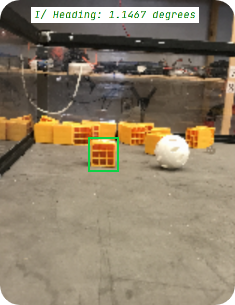
\includegraphics[width=0.95\textwidth, angle=0]{Meetings/February/02-10-22/02-10-22 1.PNG}
\caption{Our detection of a single block}
\label{fig:021022_1}
\end{figure}

\begin{figure}[htp]
\centering
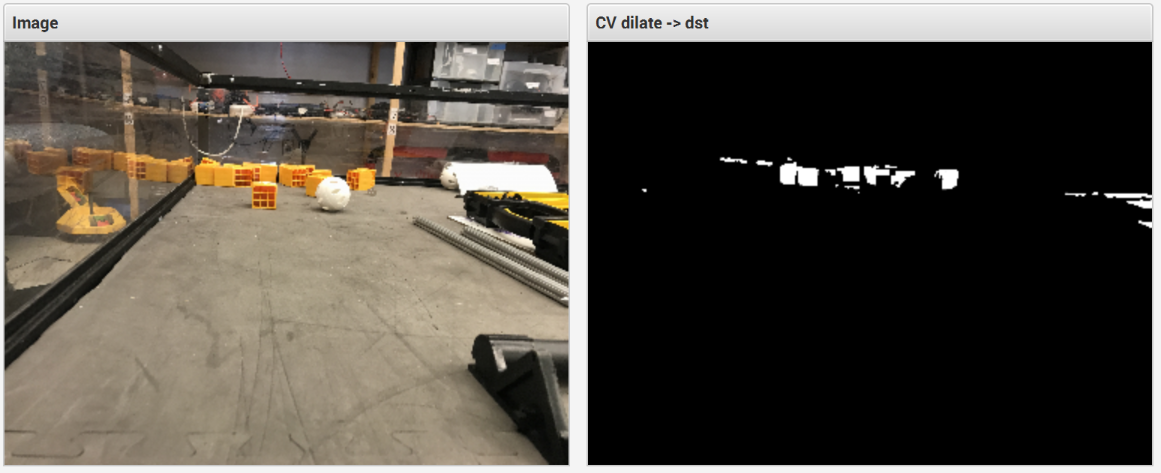
\includegraphics[width=0.95\textwidth, angle=0]{Meetings/February/02-10-22/02-10-22 2.PNG}
\caption{The large blob of blocks when tested in real life}
\label{fig:021022_2}
\end{figure}

\hhscommittee{Hardware}
\noindent\hfil\rule{\textwidth}{.4pt}\hfil
\subsubsection*{Goals}
\begin{itemize}
    \item Create second carbon fiber side plate
	\item Show other members how the process works so they can make carbon fiber parts in the future

\end{itemize} 

\noindent\hfil\rule{\textwidth}{.4pt}\hfil

\subsubsection*{Accomplishments}
After another hiatus from making our carbon fiber plates, we have finally returned to the project after more fully realizing its importance during our league competition. Although we did well in the competition, we couldn’t help but feel limited by the heavy and somewhat ineffective rev extrusion supports for the arm, which bend, making controlling the intake precisely very difficult. Although the second plate is a slightly more complex shape than the first, the process would remain generally the same. Seeing This as an opportunity, we asked some of our younger members and anyone else who was interested to come to UCF’s innovation lab and help us make the sides. 
With our carbon fiber team assembled, we started the process of creating the carbon fiber sides again, following all of the same steps and processes as last time. This time, however, many of the steps were carried out by different members who weren't there for the creation of the first sides, with some help from the members who were there. We stared by laying the mold on a glass plate, cutting all of the sections of plain weave carbon fiber then creating the border of tacky-tape around the space where the mold would be placed on the glass. Moving on to the fun part, we started adding the layers of carbon fiber onto the mold and painting them with epoxy (Figure \ref{fig:021022_4}). This step proved to be a bit trickier than on the first side, because this side has an extra protruding section where the motor will be housed. This made the layers difficult to lay completely flat, a problem we were able to remedy by adding extra epoxy on some of the parts that were bubbled up. To suck up the epoxy, we added the peel-ply and cloth layer on top of the layers of carbon fiber and epoxy (Figure \ref{fig:021022_5}). Then we cut a sheet of plastic to length, created pleats with the tacky-tape and stuck the two together to ensure a tight seal (Figure \ref{fig:021022_6}). When we turned the vacuum pump on, we noticed that the pressure was lower than it was when we created the first side. After looking around for possible holes, we found that around the raised section where the motor will sit, the plastic was pulled tighter than usual. Because of the additional height from this motor section, the bag was unable to fit perfectly over the entire mold without adding more plastic. Although the pressure was a bit lower than last time, we still decided that because it was fairly close to our previous attempt that everything would still work just as we hoped it would. Now the only thing left to do is wait for the process to be completed after around 6 hours of sitting in the vacuum bag.


\begin{figure}[htp]
\centering
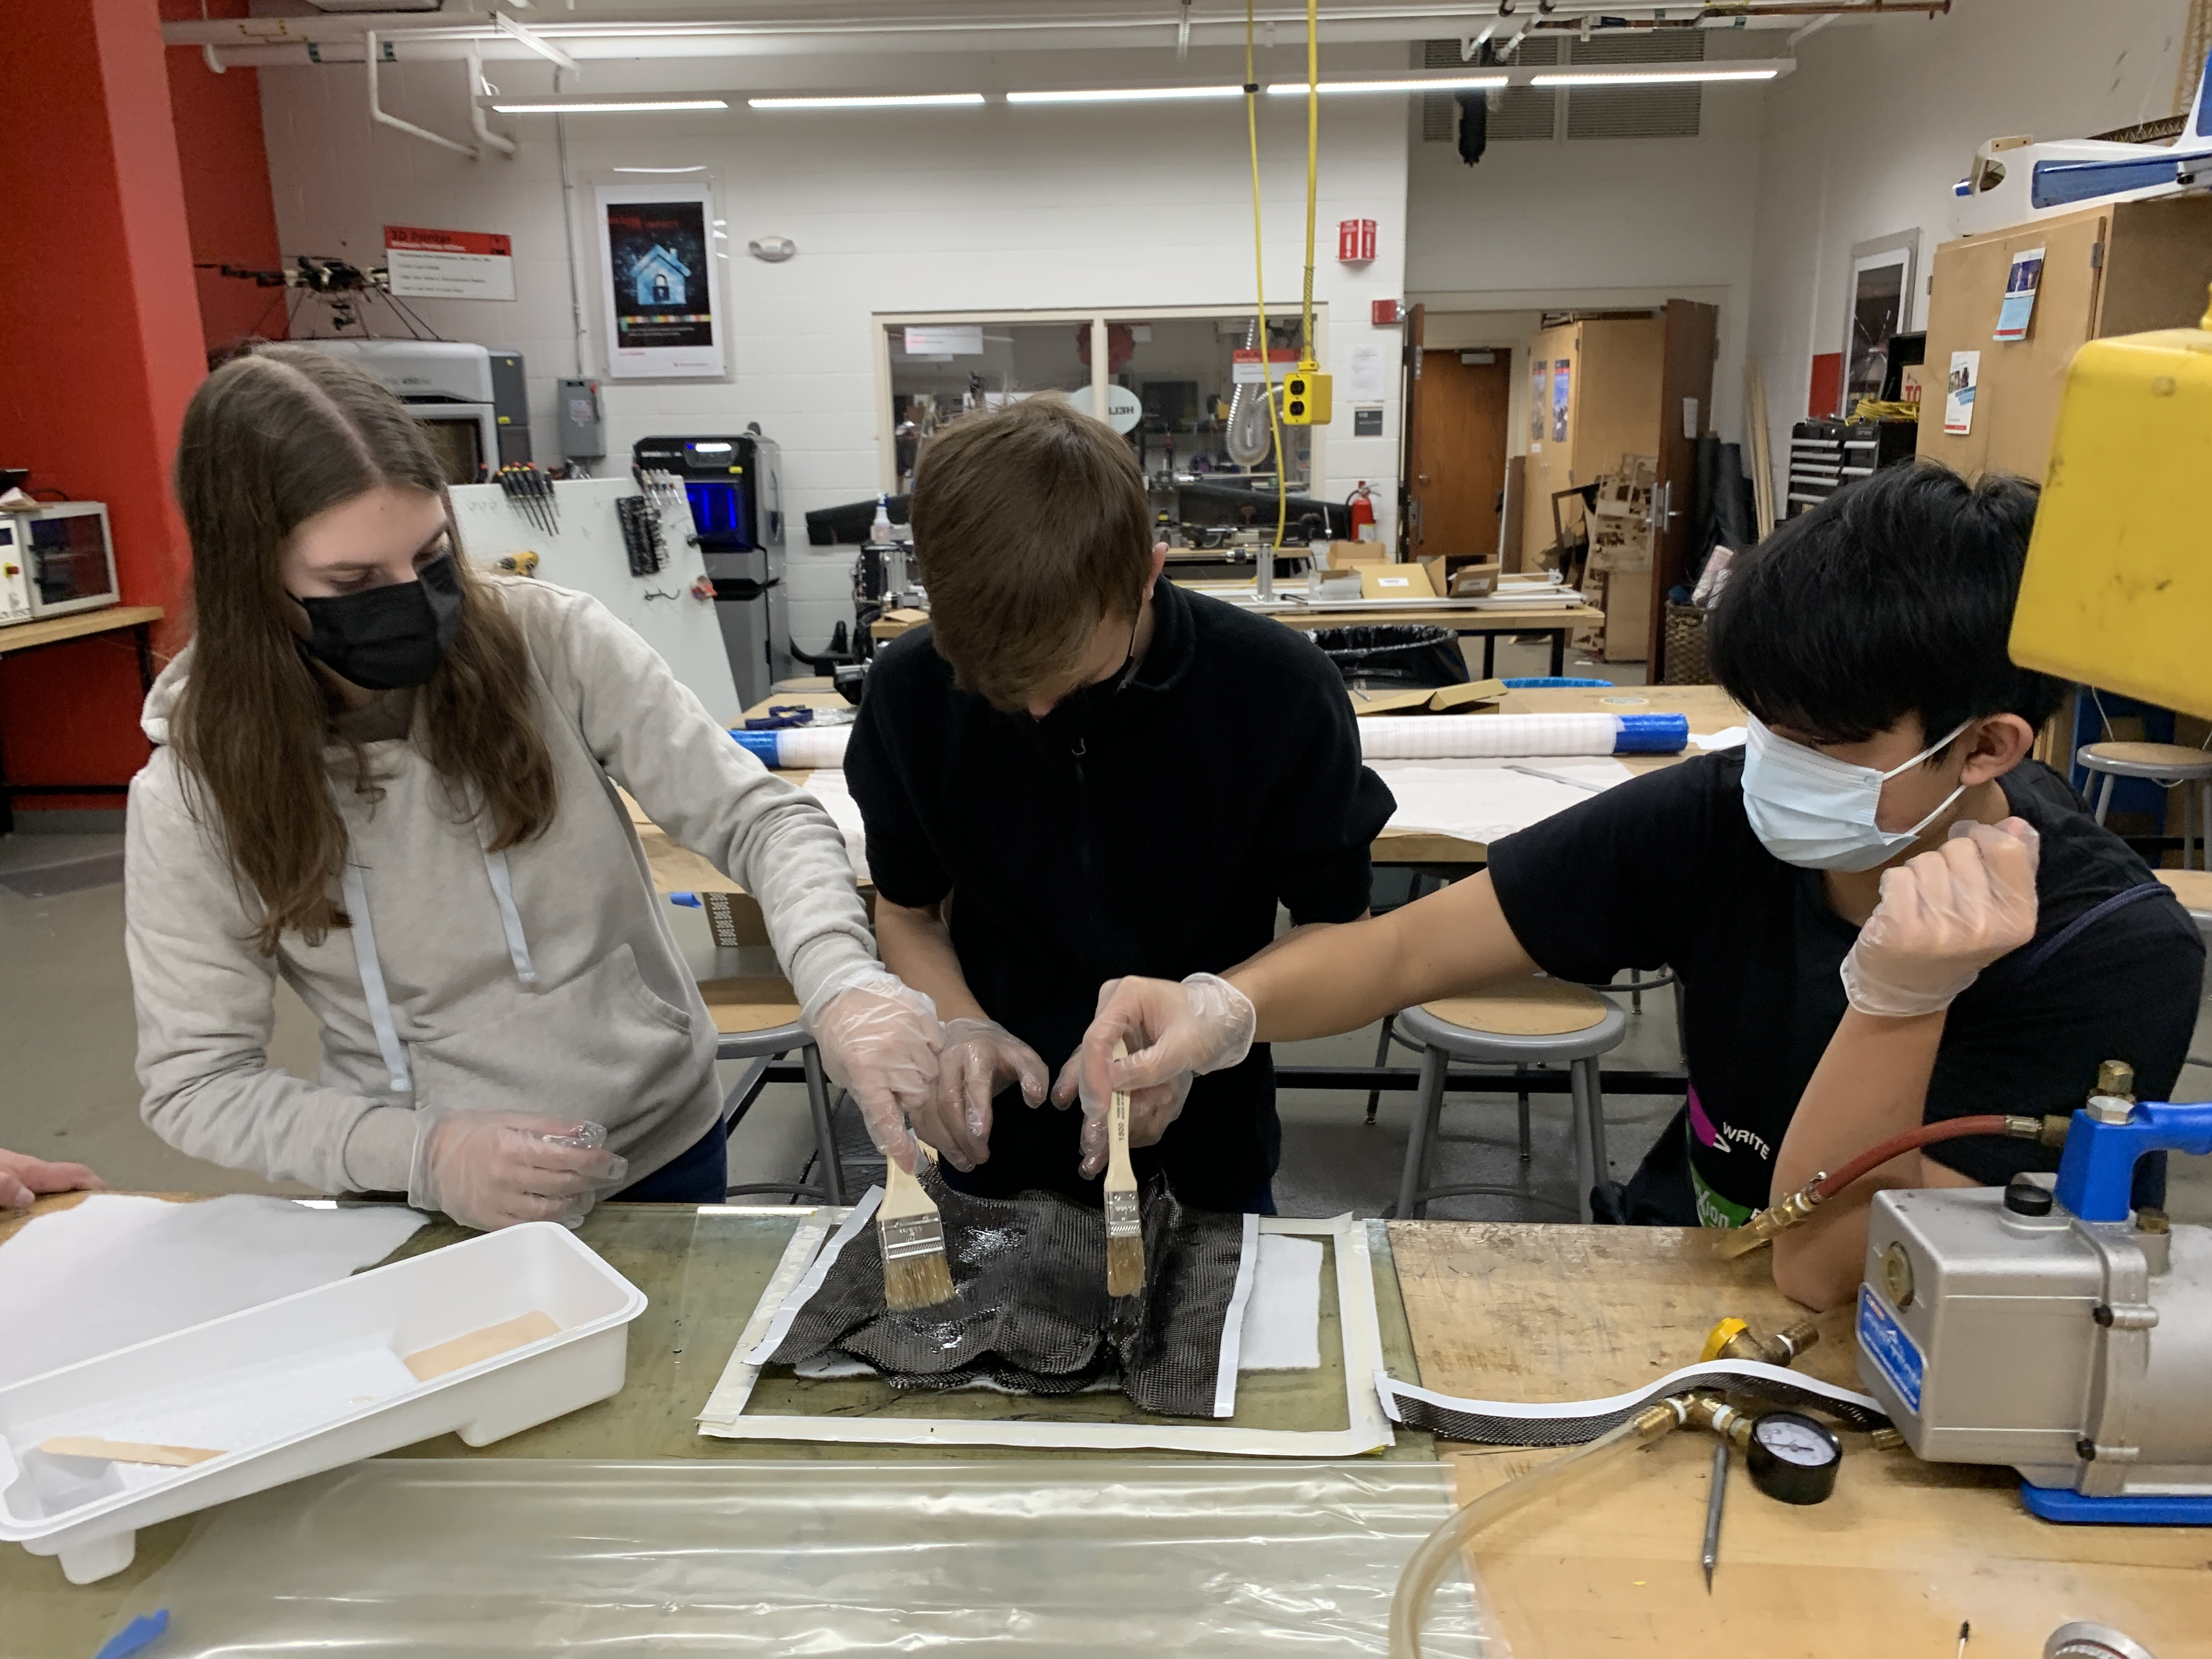
\includegraphics[width=0.95\textwidth, angle=0]{Meetings/February/02-10-22/2-10-22_Hardware_Figure1 - Nathan Forrer.JPG}
\caption{Adding layers of carbon fiber}
\label{fig:021022_4}
\end{figure}

\begin{figure}[htp]
\centering
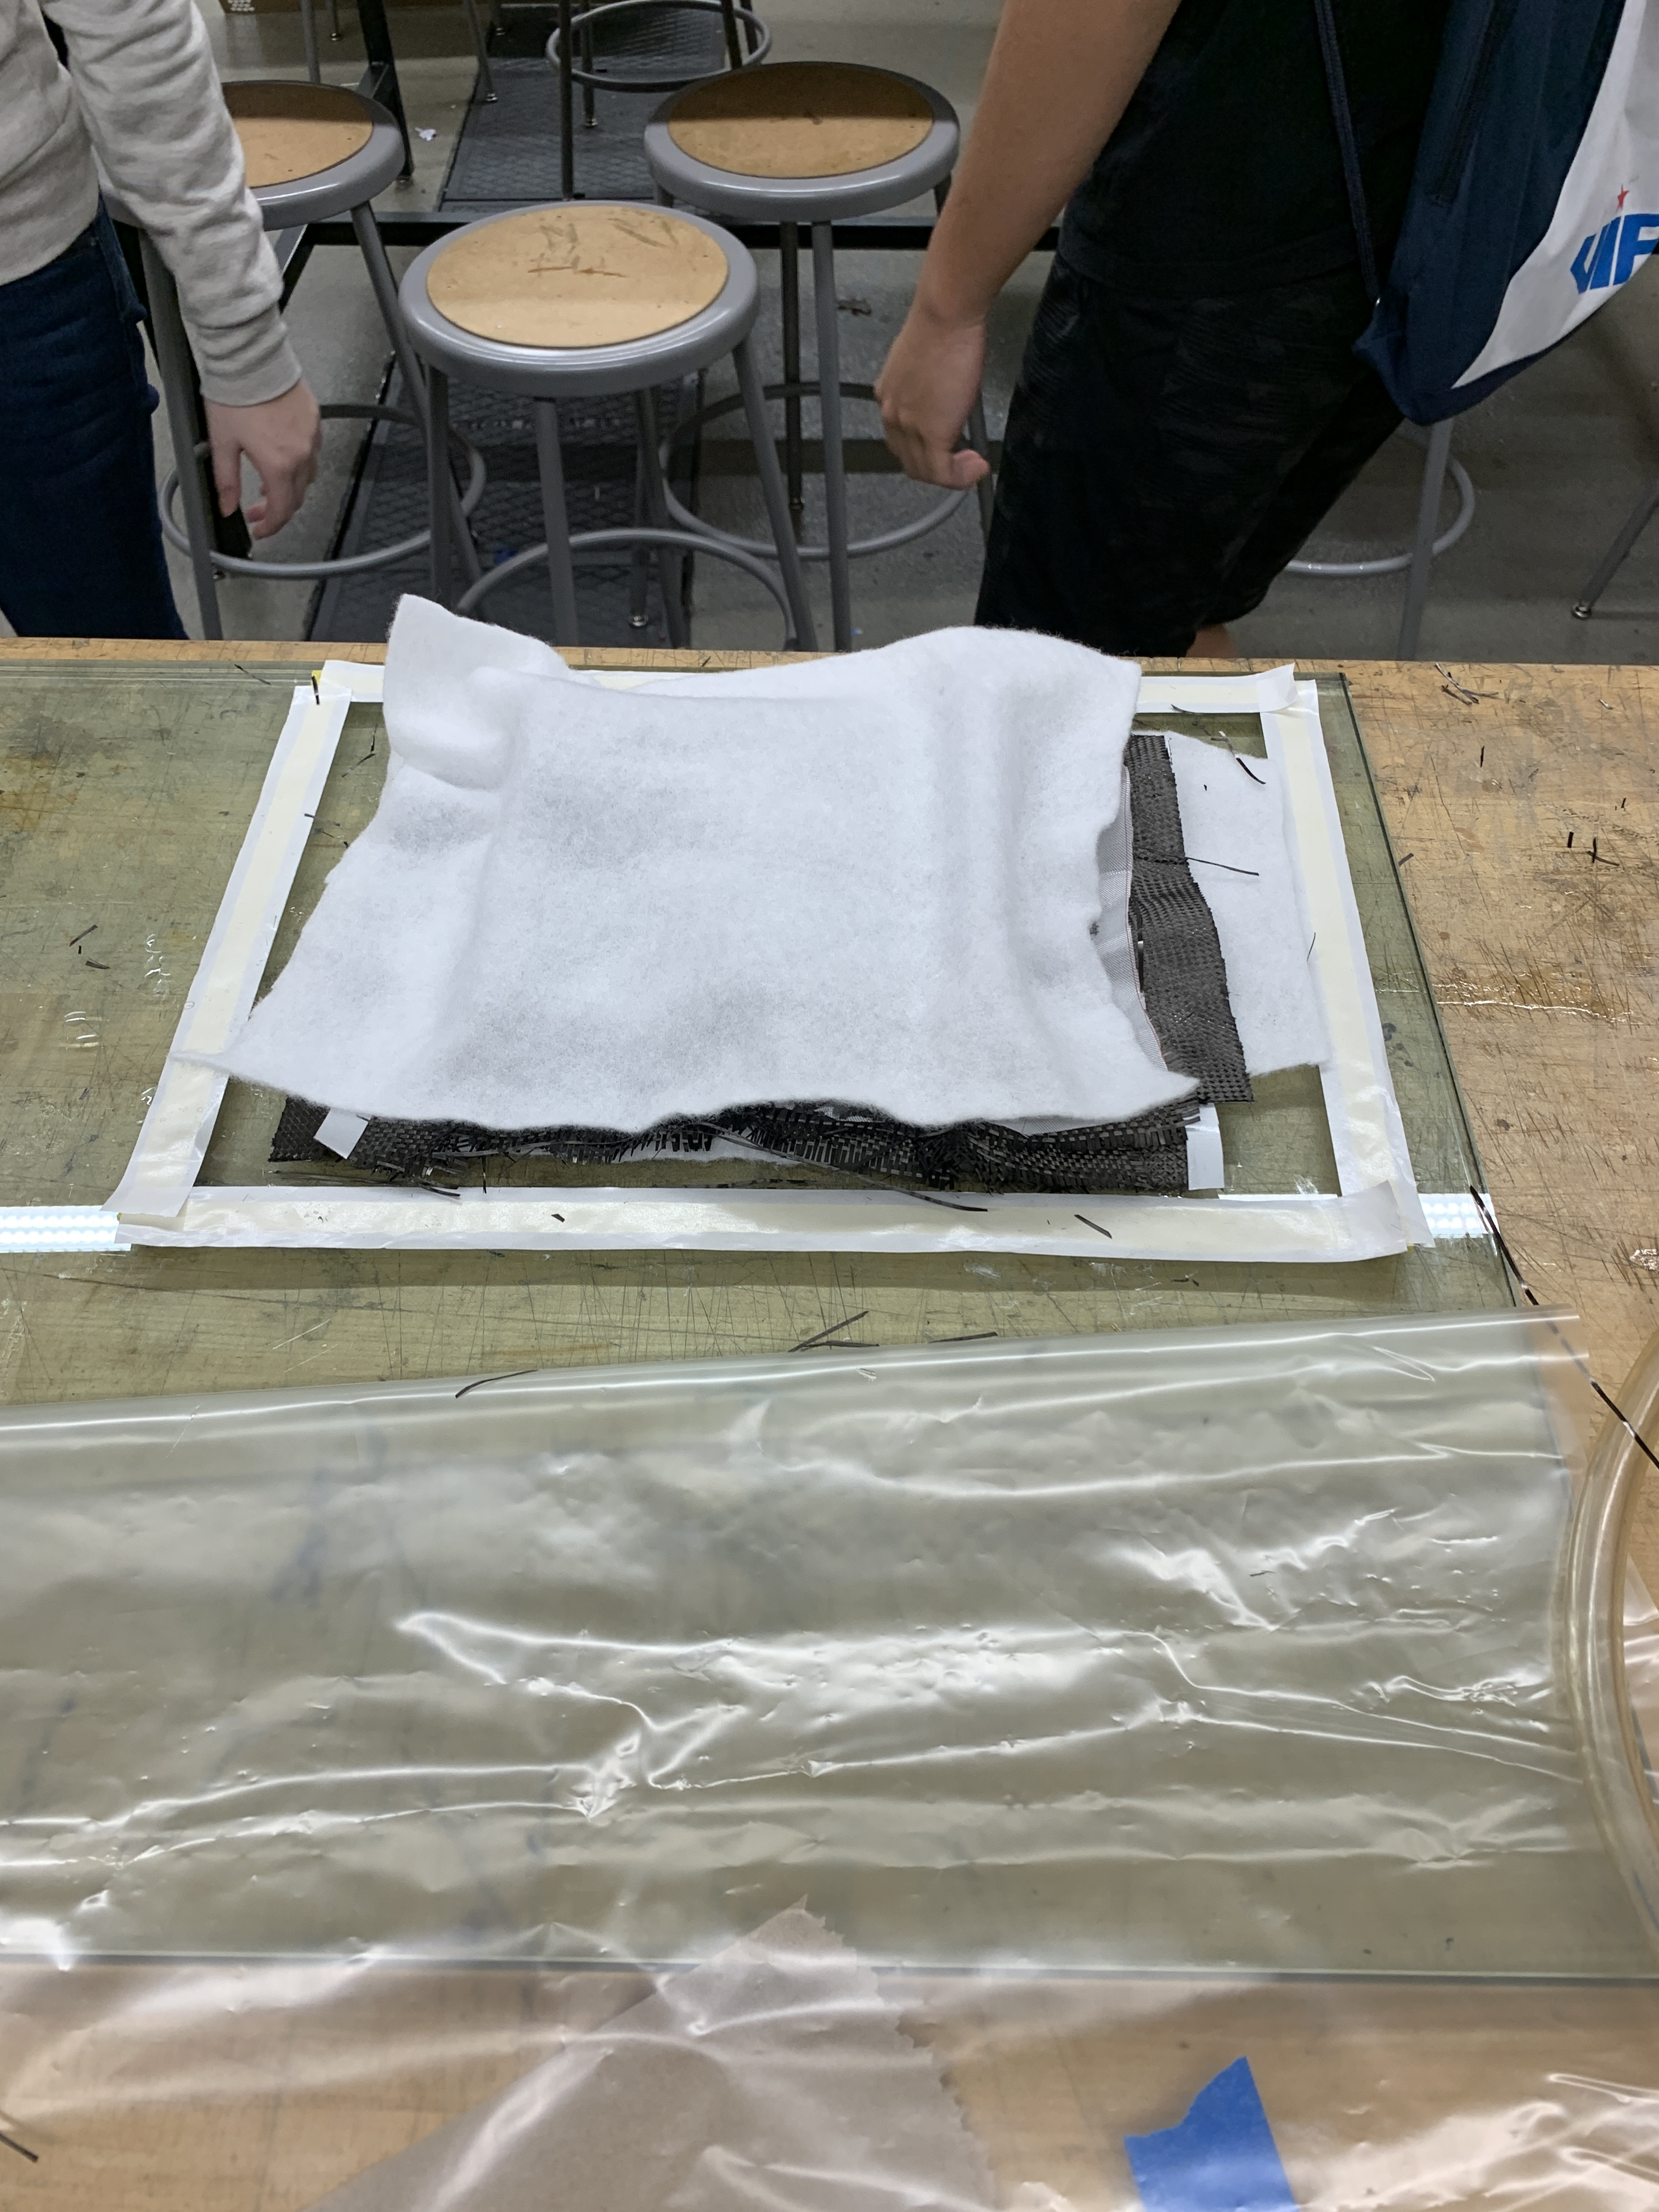
\includegraphics[width=0.95\textwidth, angle=0]{Meetings/February/02-10-22/2-10-22_Hardware_Figure2 - Nathan Forrer.JPG}
\caption{Addling peel and ply cloth layer}
\label{fig:021022_5}
\end{figure}

\begin{figure}[htp]
\centering
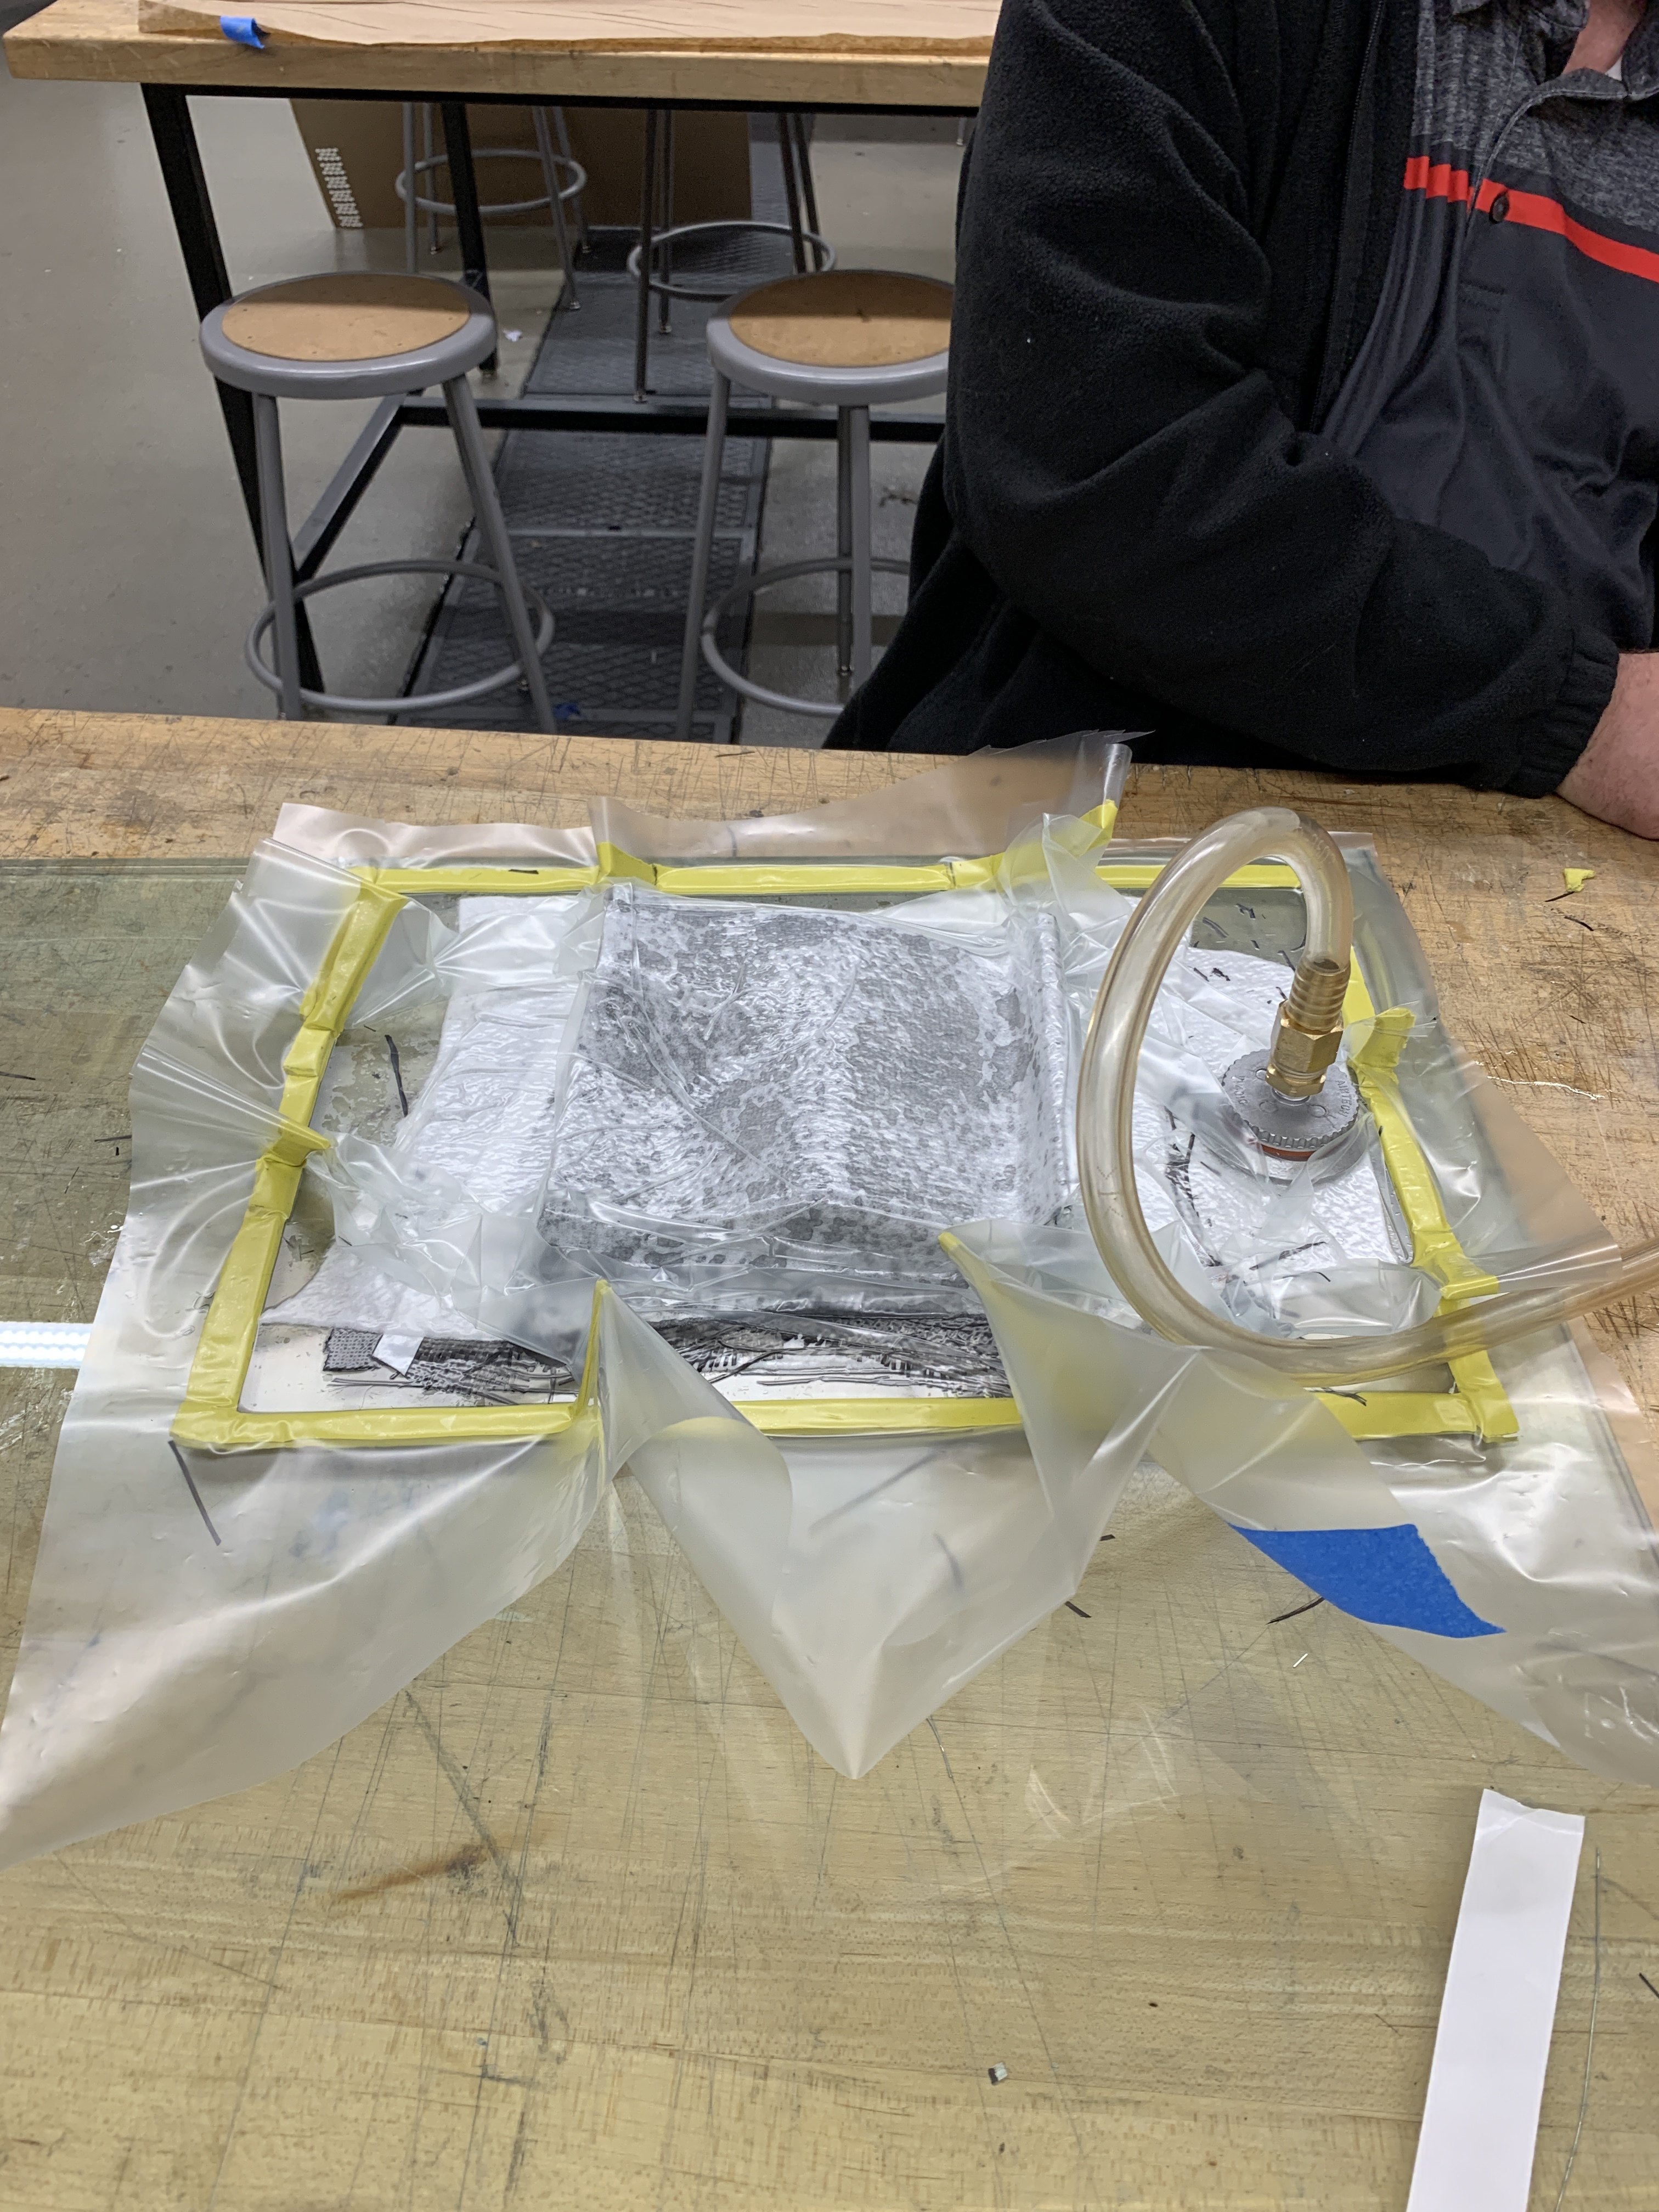
\includegraphics[width=0.95\textwidth, angle=0]{Meetings/February/02-10-22/2-10-22_Hardware_Figure3 - Nathan Forrer.JPG}
\caption{Sticking the plastic on}
\label{fig:021022_6}
\end{figure}

\whatsnext{
\begin{itemize}
    \item Implement ultrasonic sensor readings into the autonomous. 
    \item Get carbon fiber side from vacuum bag
	\item Paint over sides with epoxy
	\item Drill mounting holes in sides

\end{itemize} 
}

